\documentclass[10pt, a4paper]{article}

\usepackage[utf8]{inputenc}
\usepackage[english]{babel}
\usepackage[T1]{fontenc}
\usepackage{charter}
\usepackage{amsmath}
\usepackage{amssymb}
\usepackage{hyperref}
\usepackage{graphicx}
\usepackage{enumitem}
\usepackage{url}
\usepackage{multirow}
\usepackage{array}
\usepackage{subcaption}
\usepackage{setspace}
\usepackage{booktabs}
\usepackage[nocompress]{cite}
\usepackage{geometry}
\geometry{top=1.3cm,bottom=1.3cm,left=1.6cm,right=1.5cm}
\usepackage{xcolor}
\usepackage{listings}
\usepackage{float}

\pagestyle{plain}


\lstset{basicstyle=\ttfamily,
  showstringspaces=false,
  commentstyle=\color{red},
  keywordstyle=\color{blue},
  basicstyle=\footnotesize	
  %backgroundcolor=\xcolor{backcolour}
}



\begin{document}

\begin{center}

\textbf{Introduction to Computer Vision -- Homework 1} \\[0.1cm]

\textbf{RA192617 -- Edgar Rodolfo Quispe Condori} \\[0.1cm]
\textbf{RA192618 -- Darwin Ttito Concha} \\[0.1cm]

Institute of Computing, University of Campinas (UNICAMP) \\
Campinas-SP, Brazil, 13083-852 \\
\end{center}


\begin{itemize}
\item \textbf{beach\_2}: crater\_3, beach\_4, crater\_5 (figure\ref{fig:results_beach_2}).

\begin{figure}[H]
	\centering
	\begin{subfigure}{0.25\textwidth}
	  \centering
	  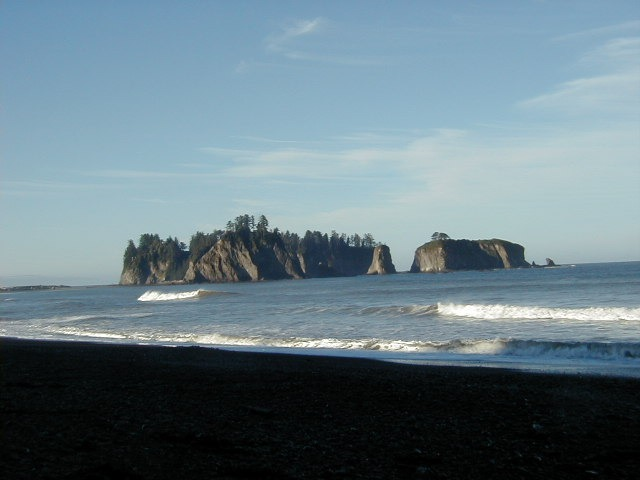
\includegraphics[width=0.9\linewidth]{../input/beach_2.jpg}
	  \caption{Query: beach\_2}
	\end{subfigure}%
	\begin{subfigure}{0.25\textwidth}
	  \centering
	  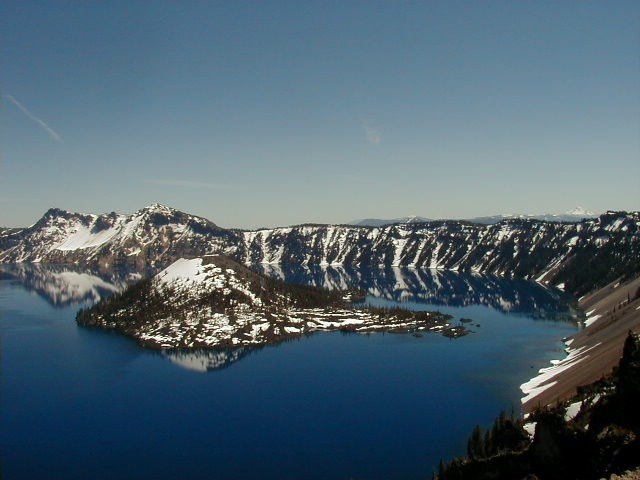
\includegraphics[width=0.9\linewidth]{../input/crater_3.jpg}
	  \caption{1st: crater\_3}
	\end{subfigure}%
	\begin{subfigure}{0.25\textwidth}
        \centering
        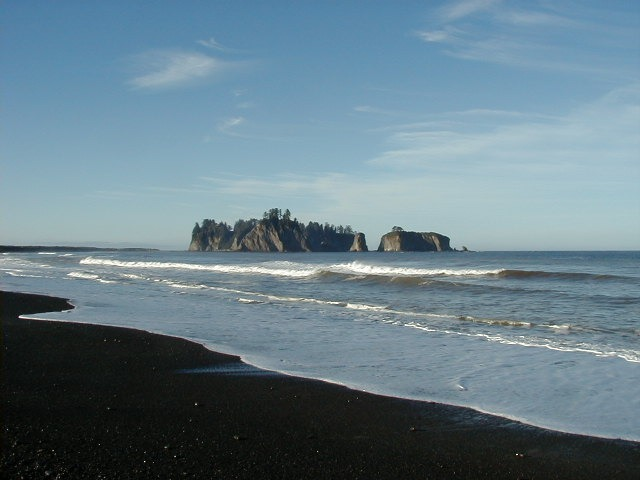
\includegraphics[width=0.9\linewidth]{../input/beach_4.jpg}
        \caption{2nd: beach\_4}
    \end{subfigure}%
    \begin{subfigure}{0.25\textwidth}
	  \centering
	  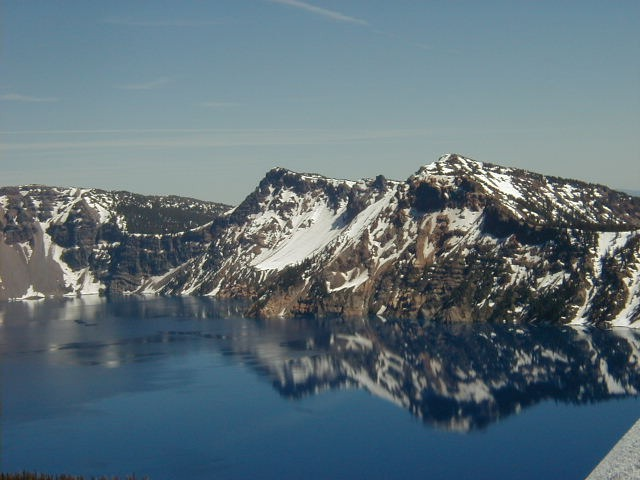
\includegraphics[width=0.9\linewidth]{../input/crater_5.jpg}
	    \caption{3th: crater\_5}
	\end{subfigure}
    \caption{Results for beach\_2}
    \label{fig:results_beach_2}
\end{figure}

\item \textbf{boat\_5}: boat\_2, cherry\_3, boat\_4 (figure \ref{fig:results_boat_5}).
\begin{figure}[H]
	\centering
	\begin{subfigure}{0.25\textwidth}
	  \centering
	  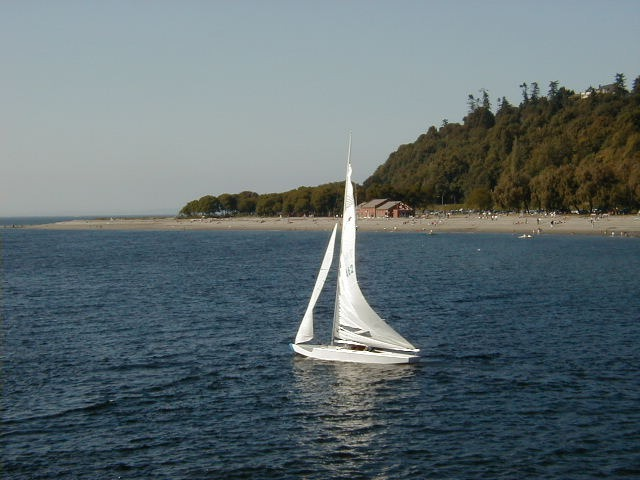
\includegraphics[width=0.9\linewidth]{../input/boat_5.jpg}
	  \caption{Query: boat\_5}
	\end{subfigure}%
	\begin{subfigure}{0.25\textwidth}
	  \centering
	  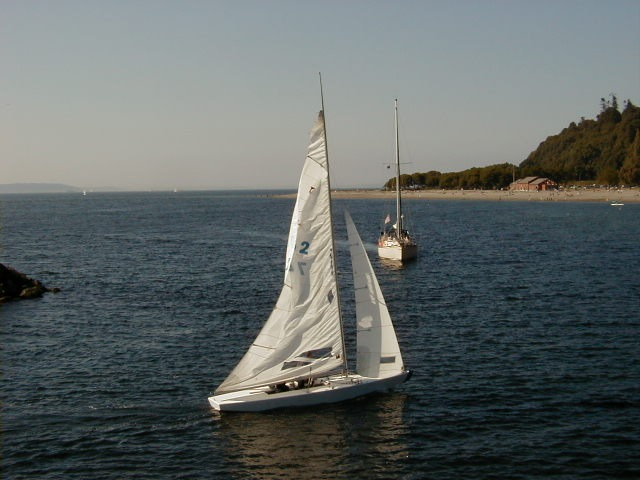
\includegraphics[width=0.9\linewidth]{../input/boat_2.jpg}
	  \caption{1st: boat\_2}
	\end{subfigure}%
	\begin{subfigure}{0.25\textwidth}
        \centering
        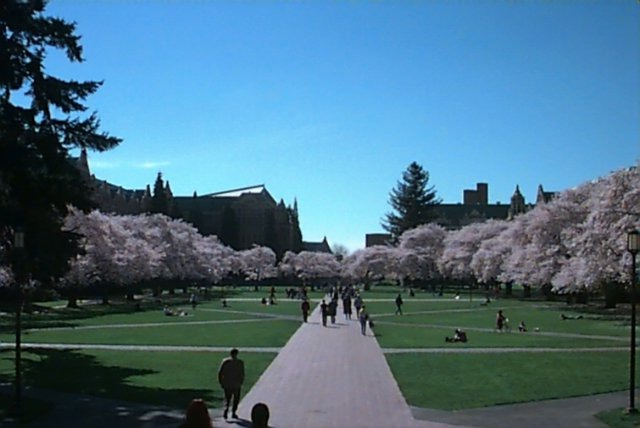
\includegraphics[width=0.9\linewidth]{../input/cherry_3.jpg}
        \caption{2nd: cherry\_3}
    \end{subfigure}%
    \begin{subfigure}{0.25\textwidth}
	  \centering
	  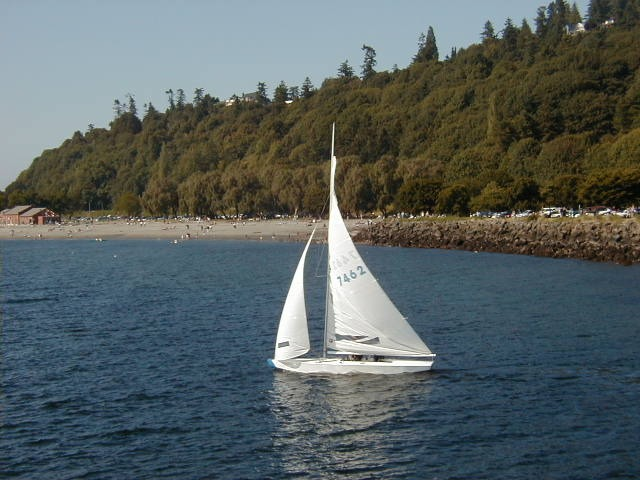
\includegraphics[width=0.9\linewidth]{../input/boat_4.jpg}
	    \caption{3th: boat\_4}
	\end{subfigure}
    \caption{Results for boat\_5}
    \label{fig:results_boat_5}
\end{figure}

\item \textbf{cherry\_3}: cherry\_2, cherry\_1, cherry\_4 (figure \ref{fig:results_cherry_3}).
\begin{figure}[H]
	\centering
	\begin{subfigure}{0.25\textwidth}
	  \centering
	  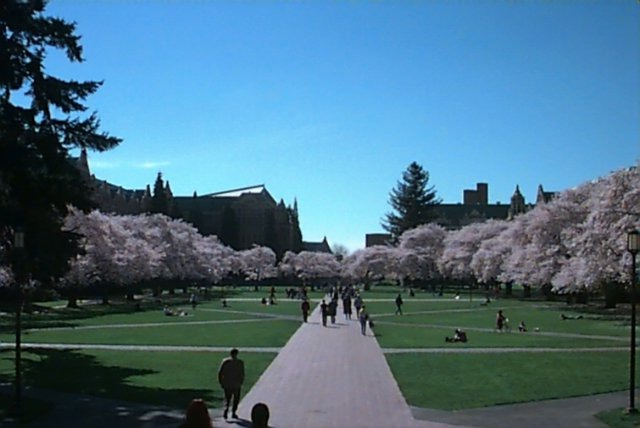
\includegraphics[width=0.9\linewidth]{../input/cherry_3.jpg}
	  \caption{Query: cherry\_3}
	\end{subfigure}%
	\begin{subfigure}{0.25\textwidth}
	  \centering
	  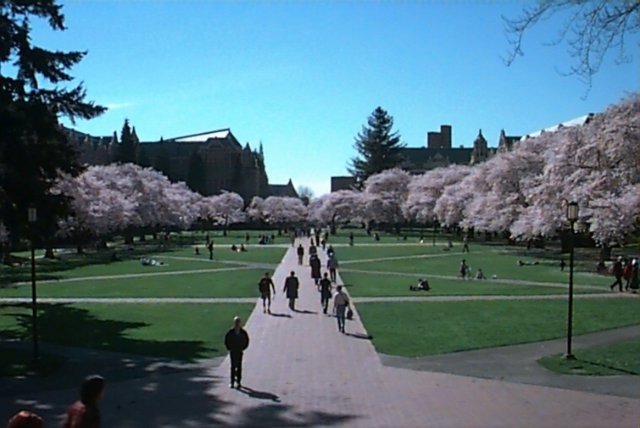
\includegraphics[width=0.9\linewidth]{../input/cherry_2.jpg}
	  \caption{1st: cherry\_2}
	\end{subfigure}%
	\begin{subfigure}{0.25\textwidth}
        \centering
        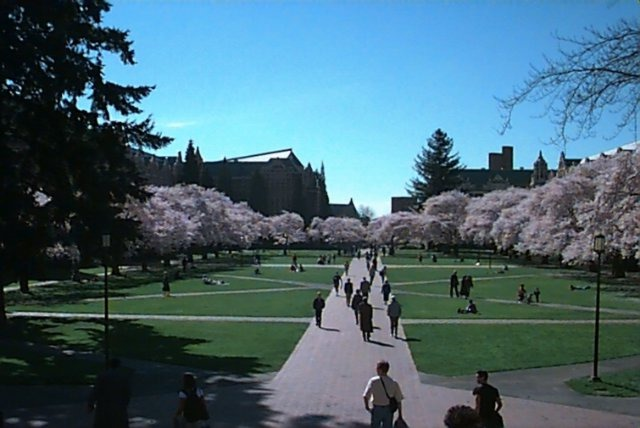
\includegraphics[width=0.9\linewidth]{../input/cherry_1.jpg}
        \caption{2nd: cherry\_1}
    \end{subfigure}%
    \begin{subfigure}{0.25\textwidth}
	  \centering
	  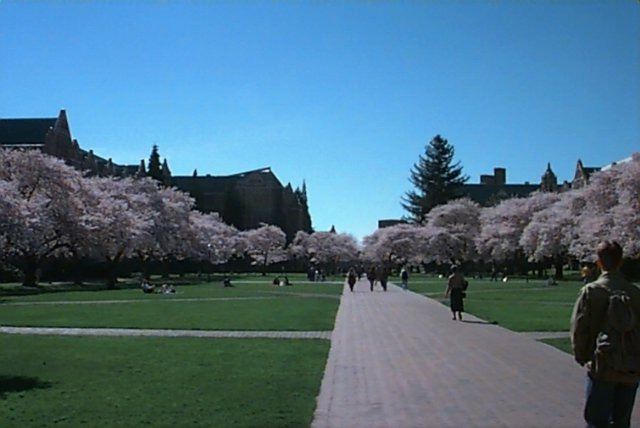
\includegraphics[width=0.9\linewidth]{../input/cherry_4.jpg}
	    \caption{3th: cherry\_4}
	\end{subfigure}
    \caption{Results for cherry\_3}
    \label{fig:results_cherry_3}
\end{figure}


\item \textbf{pond\_2}: pond\_1, pond\_3, boat\_3 (figure \ref{fig:results_pond_2}).

\begin{figure}[H]
	\centering
	\begin{subfigure}{0.25\textwidth}
	  \centering
	  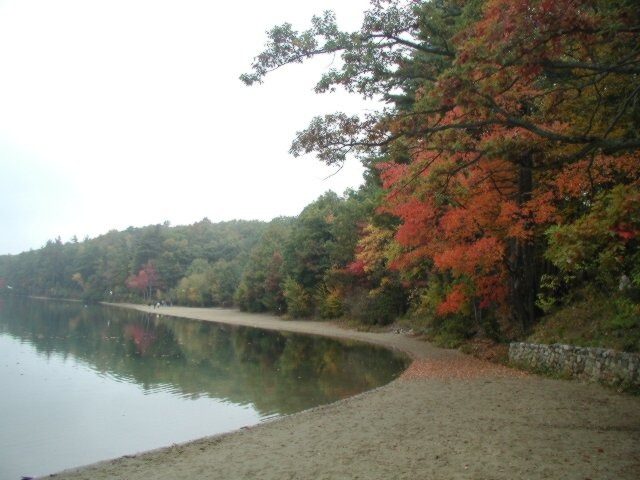
\includegraphics[width=0.9\linewidth]{../input/pond_2.jpg}
	  \caption{Query: pond\_2}
	\end{subfigure}%
	\begin{subfigure}{0.25\textwidth}
	  \centering
	  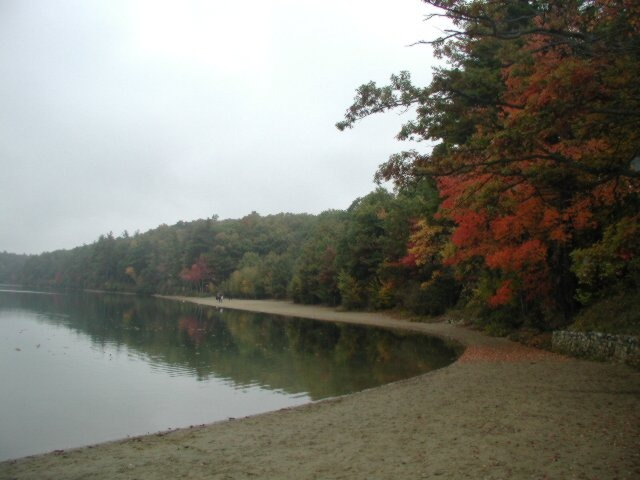
\includegraphics[width=0.9\linewidth]{../input/pond_1.jpg}
	  \caption{1st: pond\_1}
	\end{subfigure}%
	\begin{subfigure}{0.25\textwidth}
        \centering
        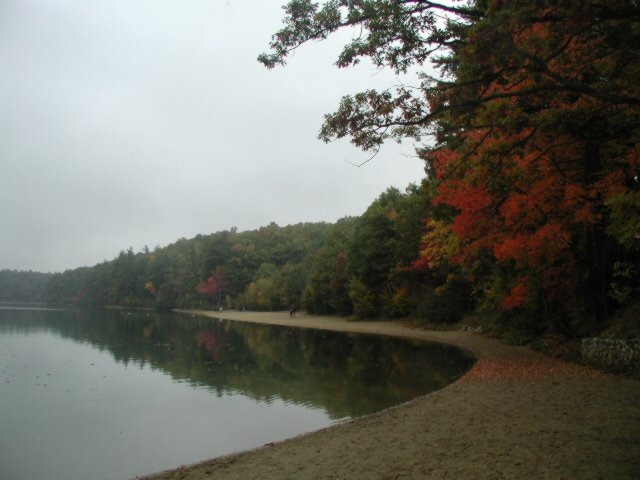
\includegraphics[width=0.9\linewidth]{../input/pond_3.jpg}
        \caption{2nd: bond\_3}
    \end{subfigure}%
    \begin{subfigure}{0.25\textwidth}
	  \centering
	  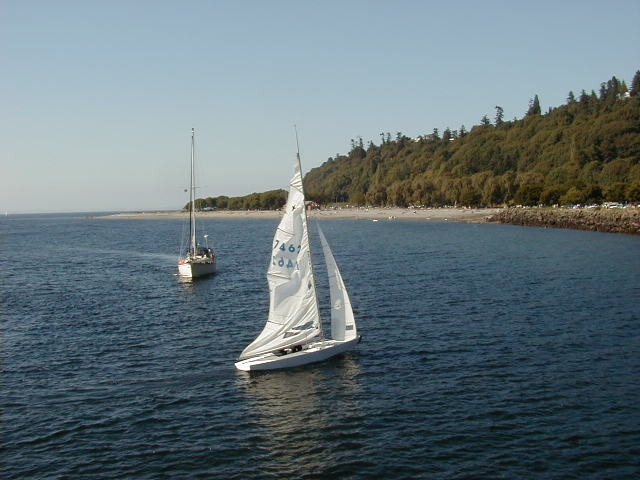
\includegraphics[width=0.9\linewidth]{../input/boat_3.jpg}
	    \caption{3th: boat\_3}
	\end{subfigure}
    \caption{Results for pond\_2}
    \label{fig:results_pond_2}
\end{figure}


\item \textbf{stHelens\_2}: stHelens\_3, stHelens\_5, stHelens\_4 (Figure \ref{fig:results_stHelens_2}).

\begin{figure}[H]
	\centering
	\begin{subfigure}{0.25\textwidth}
	  \centering
	  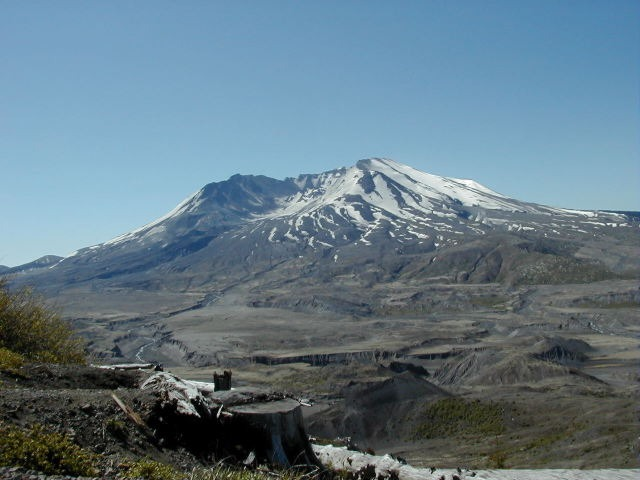
\includegraphics[width=0.9\linewidth]{../input/stHelens_2.jpg}
	  \caption{Query: stHelens\_2}
	\end{subfigure}%
	\begin{subfigure}{0.25\textwidth}
	  \centering
	  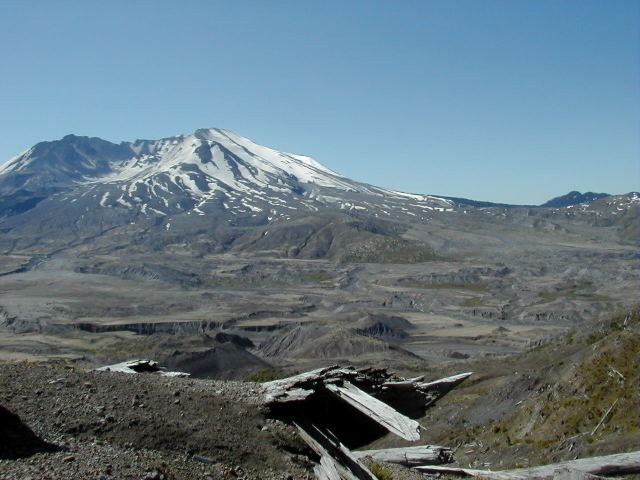
\includegraphics[width=0.9\linewidth]{../input/stHelens_3.jpg}
	  \caption{1st: stHelens\_3}
	\end{subfigure}%
	\begin{subfigure}{0.25\textwidth}
        \centering
        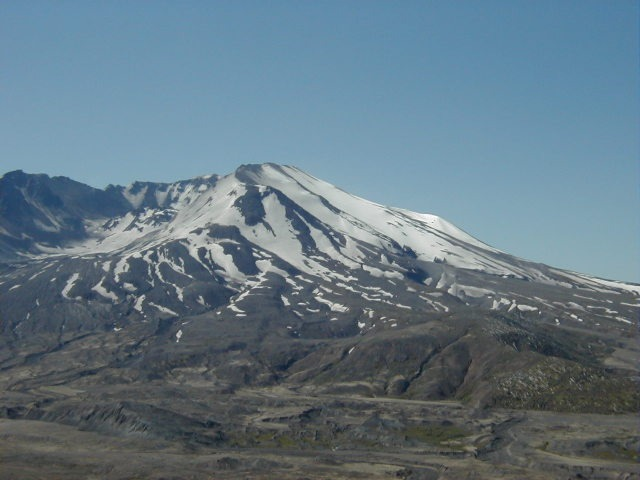
\includegraphics[width=0.9\linewidth]{../input/stHelens_5.jpg}
        \caption{2nd: stHelens\_5}
    \end{subfigure}%
    \begin{subfigure}{0.25\textwidth}
	  \centering
	  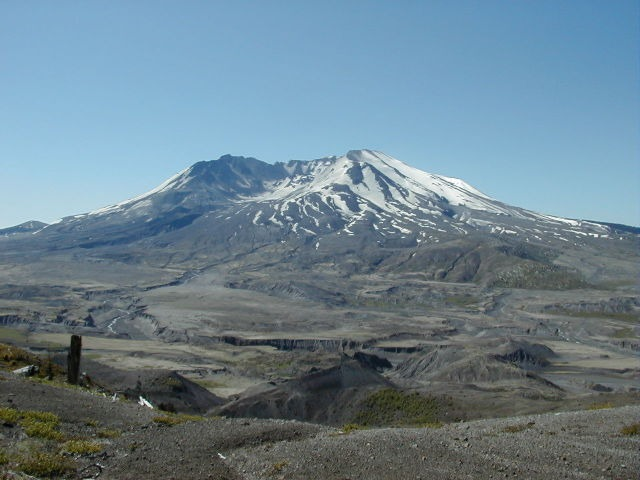
\includegraphics[width=0.9\linewidth]{../input/stHelens_4.jpg}
	    \caption{3th: stHelens\_4}
	\end{subfigure}
    \caption{Results for stHelens\_2}
    \label{fig:results_stHelens_2}
\end{figure}


\item \textbf{sunset1\_2}: sunset1\_1, sunset1\_3, beach\_4 (Figure \ref{fig:results_sunset1_2}). 

\begin{figure}[H]
	\centering
	\begin{subfigure}{0.25\textwidth}
	  \centering
	  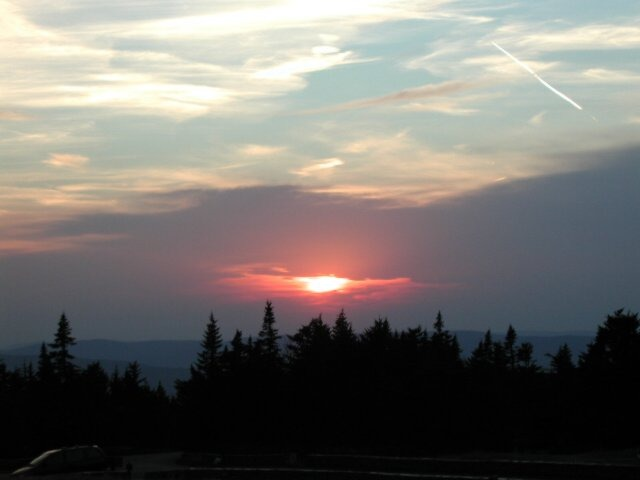
\includegraphics[width=0.9\linewidth]{../input/sunset1_2.jpg}
	  \caption{Query: sunset1\_2}
	\end{subfigure}%
	\begin{subfigure}{0.25\textwidth}
	  \centering
	  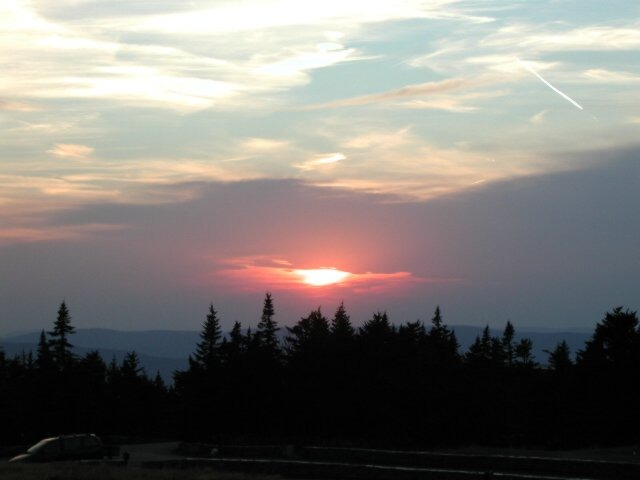
\includegraphics[width=0.9\linewidth]{../input/sunset1_1.jpg}
	  \caption{1st: sunset1\_2}
	\end{subfigure}%
	\begin{subfigure}{0.25\textwidth}
        \centering
        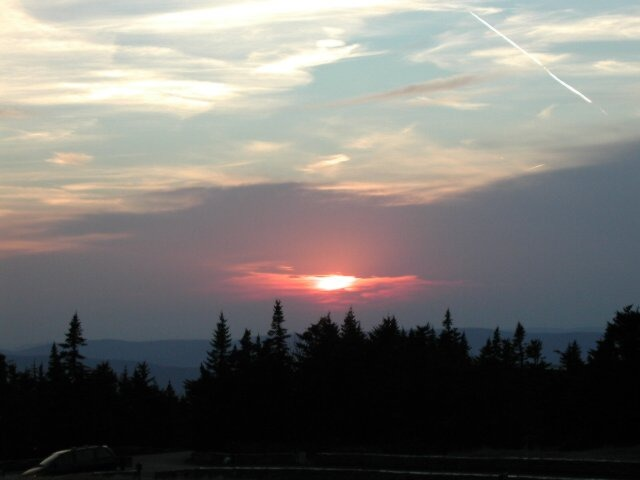
\includegraphics[width=0.9\linewidth]{../input/sunset1_3.jpg}
        \caption{2nd: sunset1\_3}
    \end{subfigure}%
    \begin{subfigure}{0.25\textwidth}
	  \centering
	  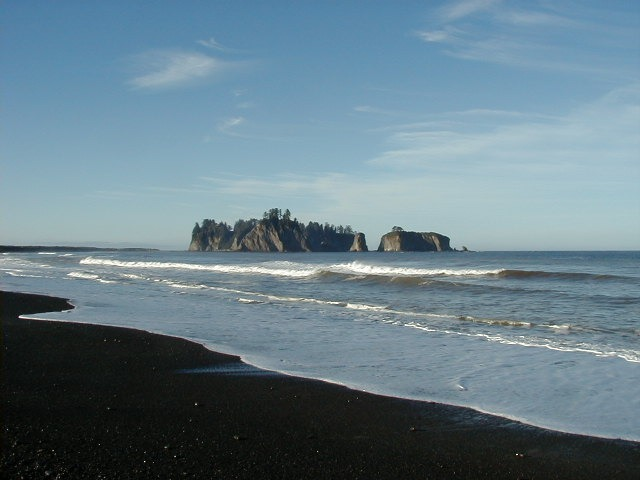
\includegraphics[width=0.9\linewidth]{../input/beach_4.jpg}
	    \caption{3th: beach\_4}
	\end{subfigure}
    \caption{Results for sunset1\_2}
    \label{fig:results_sunset1_2}
\end{figure}

\item \textbf{sunset2\_2}: sunset2\_4, sunset2\_3, beach\_2 (Figure \ref{fig:results_sunset2_2}).

\begin{figure}[H]
	\centering
	\begin{subfigure}{0.25\textwidth}
	  \centering
	  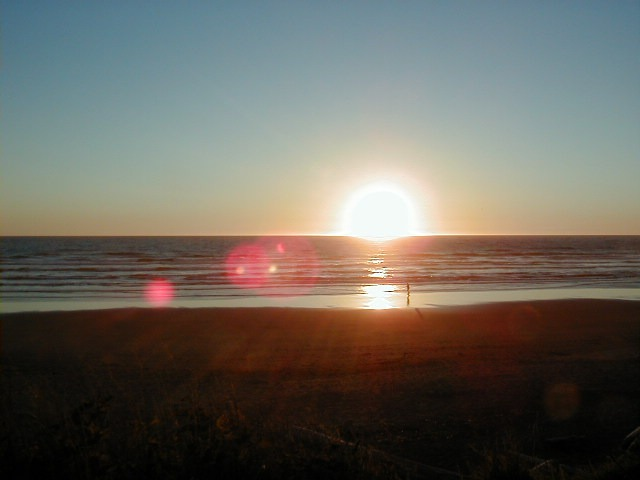
\includegraphics[width=0.9\linewidth]{../input/sunset2_2.jpg}
	  \caption{Query: sunset2\_2}
	\end{subfigure}%
	\begin{subfigure}{0.25\textwidth}
	  \centering
	  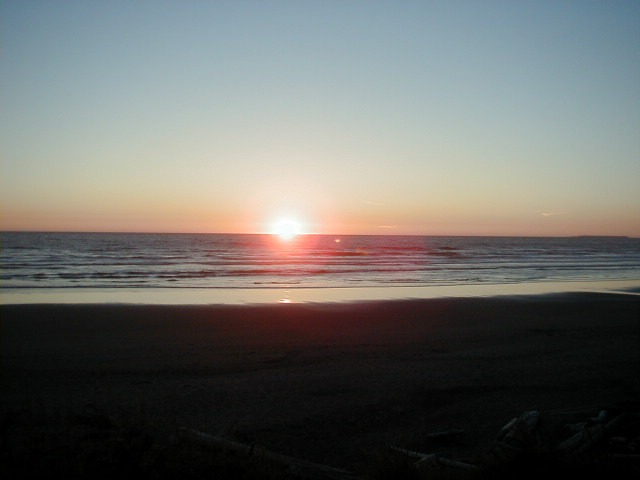
\includegraphics[width=0.9\linewidth]{../input/sunset2_4.jpg}
	  \caption{1st: sunset2\_4}
	\end{subfigure}%
	\begin{subfigure}{0.25\textwidth}
        \centering
        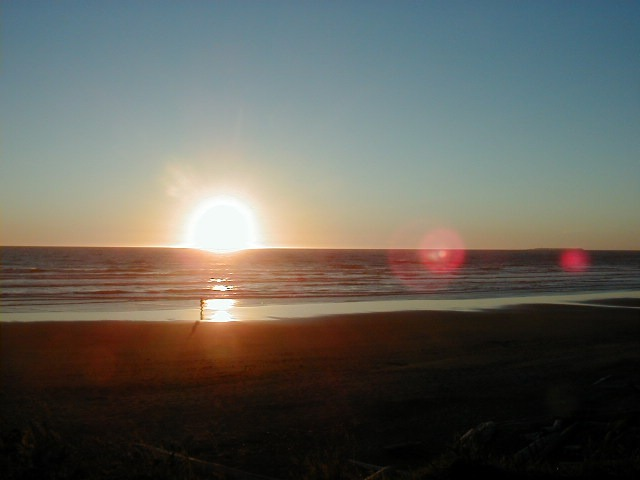
\includegraphics[width=0.9\linewidth]{../input/sunset2_3.jpg}
        \caption{2nd: sunset2\_3}
    \end{subfigure}%
    \begin{subfigure}{0.25\textwidth}
	  \centering
	  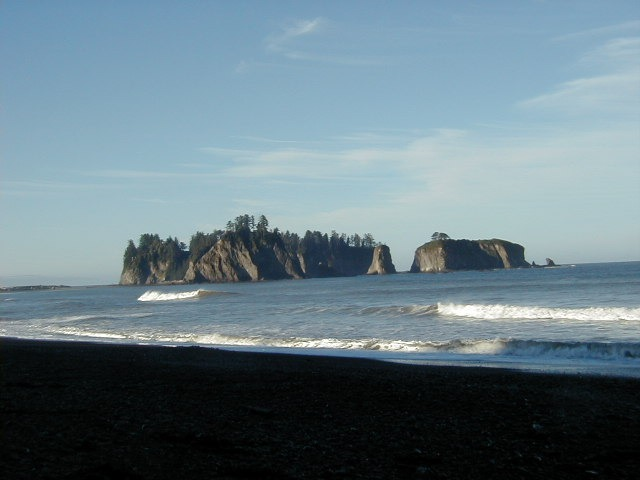
\includegraphics[width=0.9\linewidth]{../input/beach_2.jpg}
	    \caption{3th: beach\_2}
	\end{subfigure}
    \caption{Results for sunset2\_2}
    \label{fig:results_sunset2_2}
\end{figure}

\end{itemize}



\bibliographystyle{unsrt}
\bibliography{report}

\end{document}
